% ::setlocal makeprg=cd\ report\ &&\ pdflatex\ -interaction=batchmode\ main.tex\ &&\ xdg-open\ main.pdf\ &&\ exit

\documentclass[a4paper, titlepage]{article}
\newcommand{\Punit}[0]{\frac{\unit{\mega\electronvolt}}{c^2 \unit{\femto\cubic\meter}}}
\newcommand{\Sh}[0]{Schwarzschild }

%\verb|\stretchto| with aspect ratio limit of 4.4

\usepackage[T1]{fontenc}
\usepackage[utf8]{inputenc}
\usepackage[italian]{babel}
%\usepackage[hashEnumerators,smartEllipses]{markdown}
\usepackage{mathtools}
\usepackage{siunitx} % Load siunitx first
\usepackage{physics} % Load physics after siunitx
%\usepackage{amsmath} %mathtools loads amsmath too!!
\usepackage{amssymb}
\usepackage[overload]{empheq}
\usepackage{listings}
\usepackage{tabularx}
\usepackage{textcomp}
\usepackage{multirow}
\usepackage{multicol}
\usepackage{booktabs}
\usepackage{graphicx}
\usepackage{floatflt}
\usepackage{epsfig}
\usepackage{pstricks}
\usepackage{subcaption}
\usepackage[labelfont=bf, font=scriptsize]{caption}
\usepackage[italian]{varioref}
\usepackage[suftesi,write]{frontespizio}
\usepackage{xcolor}
\usepackage{caption}
\usepackage{pgfplots}
\usepackage{comment}
\usepackage{bm}            % special bold-math package. usge: \bm{mathsymbol}
\usepackage{array}
\usepackage{lipsum}
\usepackage{csquotes}
\usepackage{biblatex}
%\addbibresource{sample-paper.bib}
\usepackage[colorlinks=true]{hyperref}  % this package should be added after all others.
\pgfplotsset{compat=1.16}
\usepackage[text={15.5cm,23.5cm},centering,heightrounded]{geometry}
\DeclareCaptionType{eq_caption}[Equazione][Elenco delle equazioni]

\definecolor{mygreen}{rgb}{0,0.6,0}
\definecolor{mygray}{rgb}{0.5,0.5,0.5}
\definecolor{mymauve}{rgb}{0.58,0,0.82}

\lstset{ 
  backgroundcolor=\color{white},   % choose the background color; you must add \usepackage{color} or \usepackage{xcolor}; should come as last argument
  basicstyle=\footnotesize,        % the size of the fonts that are used for the code
  breakatwhitespace=false,         % sets if automatic breaks should only happen at whitespace
  breaklines=true,                 % sets automatic line breaking
  captionpos=b,                    % sets the caption-position to bottom
  commentstyle=\color{mygreen},    % comment style
  deletekeywords={...},            % if you want to delete keywords from the given language
  escapeinside={\%*}{*)},          % if you want to add LaTeX within your code
  extendedchars=true,              % lets you use non-ASCII characters; for 8-bits encodings only, does not work with UTF-8
  firstnumber=1,                   % start line enumeration with line 1000
  frame=single,	                 % adds a frame around the code
  keepspaces=true,                 % keeps spaces in text, useful for keeping indentation of code (possibly needs columns=flexible)
  keywordstyle=\color{blue},       % keyword style
  %language=Octave,                % the language of the code
  morekeywords={*,...},            % if you want to add more keywords to the set
  numbers=left,                    % where to put the line-numbers; possible values are (none, left, right)
  numbersep=5pt,                   % how far the line-numbers are from the code
  numberstyle=\tiny\color{mygray}, % the style that is used for the line-numbers
  rulecolor=\color{black},         % if not set, the frame-color may be changed on line-breaks within not-black text (e.g. comments (green here))
  showspaces=false,                % show spaces everywhere adding particular underscores; it overrides 'showstringspaces'
  showstringspaces=false,          % underline spaces within strings only
  showtabs=false,                  % show tabs within strings adding particular underscores
  stepnumber=1,                    % the step between two line-numbers. If it's 1, each line will be numbered
  stringstyle=\color{mymauve},     % string literal style
  tabsize=2,	                   % sets default tabsize to 2 spaces
  title=\lstname                   % show the filename of files included with \lstinputlisting; also try caption instead of title
}


% To stretch integrals
\usepackage{scalerel}[2016-12-29]
\def\stretchint#1{\vcenter{\hbox{\stretchto[440]{\displaystyle\int}{#1}}}}
\def\scaleint#1{\vcenter{\hbox{\scaleto[3ex]{\displaystyle\int}{#1}}}}
\def\bs{\mkern-12mu} % and set amount of backspacing for lower limit of integration

%\begin{frontespizio}
    \Universita{Trento} % CTT
    \Logo{Figures/logo_unitn} % CTT
    \Divisione{Fisica Computazionale} % CTT
    \Corso[Laurea Triennale]{Fisica} % CTT, a meno che non cambi la denominazione del corso
    \Annoaccademico{2023-2024}
    \Titoletto{Progetto Finale} % CTT
    \Titolo{Calcolo redshift nell'emissione di fotoni da una stella di neutroni\\ }
    \Sottotitolo{\today}
    \Candidato[227552]{Federico De Paoli, \textsf {federico.depaoli@studenti.unitn.it}}
    \NRelatore{Docente}{} % CTT
    \Relatore{Prof. Alessandro Roggero} % CTT, a meno che non sia cambiato il Prof.
\end{frontespizio}
\IfFileExists{\jobname-frn.pdf}{}{%
\immediate\write18{pdflatex \jobname-frn}} % ASSOLUTAMENTE CTT, è il comando che materialmente vi genera il frontespizio.

\newpage



\begin{document}

\tableofcontents
\newpage

\section{Introduzione}
Studiamo la stabilità delle stelle di neutroni in regime relativistico
considerando 3 possibili equazioni di stato per la materia.
Una volta risolte le equazioni è possibile ottenere l'espressione del potenziale
gravitazione della stella e calcolare l'effetto sulla radiazione emessa dalla
stella.


Viene calcolata la radianza per ogni stella a 3 distanze diverse e la potenza
totale di emissione in funzione della distanza dalla stella.
Viene quindi calcolata la temperatura apparente delle 3 stelle più massive in
funzione di quella effettiva e poi viene studiata la temperatura apparente in 
funzione della pressione centrale della stella.


\section{Stabilità}

Le equazioni che descrivono la stabilità di una stella in funzione della massa
($m$) e della pressione ($P$) sono quelle di Tolman-Oppenheimer-Volkoff
\begin{subequations}
\begin{align}[left = {\empheqlbrace}]
    \dv[]{P(r)}{r} &= - G \frac{m(r) \epsilon (r)}{r^2 c^2}
    \left(1 + \frac{P(r)}{\epsilon (r)} \right)
    \left(\ + \frac{4 \pi r^3 P(r)}{m(r) c^2} \right)
    \left(1 - \frac{2 G m(r)}{r c^2} \right)^{-1} \label{eq:P_corr} \\
    %
    \dv[]{m(r)}{r} &= 4 \pi r^2 \frac{\epsilon (r)}{c^2} \label{eq:m_corr} \\
    %
    \dv[]{\Phi(r)}{r} &= - \frac{1}{P(r) + \epsilon (r)} \dv[]{P(r)}{r}
    \label{eq:Phi_corr}
\end{align}
\label{eq:sistema_corr}
\end{subequations}

Dove la terza equazione è l'equazione disaccoppiata e descrive il potenziale gravitazionale della stella.
Usiamo 3 diverse densità di energia per la materia della stella (eq. \ref{eq:energia23} viene presa con due coppie di valori diversi di $\Gamma$ e $K$):
\begin{subequations}
\begin{align}
    \epsilon_1 (n) &= \mu c^2 n
    + a n_0 \left( \frac{n}{n_0} \right) ^{\alpha + 1}
    + b n_0 \left( \frac{n}{n_0} \right) ^{\beta + 1} \label{eq:energia1} \\
    \epsilon_{2/3} (n) &= \mu c^2n+Kc^2n^\Gamma \label{eq:energia23}
\end{align}
\end{subequations}
\begin{equation}
    \text{con} \quad a = 13.4 \unit{\mega\electronvolt\per\femto\cubic\meter} \ , \quad
    \alpha = 0.514, \quad
    b = 5.62 \unit{\mega\electronvolt\per\femto\cubic\meter} \ , \quad
    \beta = 2.436 \ , \quad
    n_0 = 0.16 \unit{\per\femto\cubic\meter}
\end{equation}

dove $n$ è la densità numerica, $\mu$ la massa del neutrone e quindi
$\rho = \mu n$ è la densità di massa.

Visto che la densità di energia è in funzione di $\rho$ e le incognite del
sistema \ref{eq:sistema_corr} sono $P$ e $m$ possiamo scrivere la densità di
energia in funzione di $P$ e $m$ partendo dalla relazione termodinamica

\begin{subequations}
    \label{eq:eps(r)}
    \begin{align}[left = {P = - \dv[]{E}{V} \Rightarrow \empheqlbrace}]
        P &= \alpha a n_0 \left( \frac{n}{n_0} \right)^{\alpha + 1}
        + \beta b n_0 \left( \frac{n}{n_0} \right)^{\beta + 1}
        && \text{per } \epsilon_1 \label{eq:eps(r)1} \\
        n &= \left( \frac{P}{K(\Gamma - 1) c^2} \right)^{1 / \Gamma}
        && \text{per } \epsilon_{2/3} \label{eq:eps(r)23}
    \end{align}
\end{subequations}

Nel primo caso (eq. \ref{eq:eps(r)1}) non è stato possibile invertire
l'equazione per trovare $n$ in funzione di $P$ e $m$ quindi utilizzeremo un
metodo numerico per trovare $n$ di volta in volta.

Facciamo le seguenti sostituzioni per rendere le variabili adimensionali e con
valori più vicini a 0.

\begin{equation*}
    m=M_0\hat m, \quad 
    r=R_0\hat r, \quad 
    P=P_0\hat P, \quad
    \rho=\rho_0 \hat{\rho}, \quad
    K = \hat{K}\frac{\mu^\Gamma}{\rho_0^{\Gamma-1}},
\end{equation*}

\begin{subequations}
    \begin{align}[left = {\empheqlbrace}]
        \dv[]{\hat P}{\hat r} &=
        - \frac{(\hat P + \hat{\epsilon})(\hat m + \hat r^3 \hat P)}
        %
        {\hat r^2-2\hat m\hat r} \label{eq:P_ad} \\
        \dv[]{\hat m}{\hat r} &= \hat r^2 \hat{\epsilon} \label{eq:m_ad} \\
        %
        \dv[]{\Phi}{\hat r} &= - \frac{1}{\hat P + \hat{\epsilon}}
        \dv[]{\hat P}{\hat r} \label{eq:Phi_ad}
    \end{align}
    \label{eq:sistema_adim}
\end{subequations}

Otteniamo il sistema \ref{eq:sistema_adim}, dove le densità di energia sono

\begin{subequations}
\begin{align}
    \hat \epsilon_1 (\hat n) &= \hat n + \frac{a n_0}{P_0} ~ \hat n^{\alpha + 1}
    + \frac{b n_0}{P_0} ~ \hat n^{\beta + 1}
    \quad \quad {\rm dove~vale} \quad
    \hat P = \frac{\alpha a n_0}{P_0} ~ \hat n^{\alpha + 1}
    + \frac{\beta b n_0}{P_0} ~ \hat n^{\beta + 1} \label{eq:e1_ad} \\
    %
    \hat \epsilon_2 (\hat P)
    &= \left(\frac{\hat P}{\hat K (\Gamma - 1)} \right)^{1/\Gamma}
    + \frac{\hat P}{\Gamma - 1} \label{eq:e23_ad}
\end{align}
\end{subequations}

Nel caso di $\epsilon_1$ non è possibile invertire la relazione $P(n)$ e quindi
si utilizzerà un metodo numerico.
Per le politropiche $\epsilon_2$ e $\epsilon_3$ si utilizzano i seguenti valori

\begin{table}[h]
    \centering
    \begin{tabular}{c|c|c} 
         & $\hat K$ & $\Gamma$ \\
        \hline
        $\epsilon_2$ & $5 / 3$ & $0.05$ \\
        \hline
        $\epsilon_3$ & $2.54$ & $0.01$ \\
    \end{tabular}
\end{table}

Infine, i valori delle costati utilizzate per definire le variabili
adimensionali sono i seguenti

\begin{equation}
    M_0 = 12.655756 M_\odot \quad R_0 = 20.06145 \unit{\kilo\meter} \quad
    \epsilon = P_0 = \rho_0 c^2 = n_0 \mu c^2 = 150.174 \Punit
    \label{eq:val_cost}
\end{equation}

Per il potenziale gravitazionale $\Phi$ si può inoltre trovare una soluzione
analitica all'esterno della stella che possiamo mettere in forma adimensionale
(eq. \ref{eq:Phi_ext}), dove $\hat{M}$ e $\hat R$ sono rispettivamente la massa
totale e il raggio della stella in forma adimensionale.

\begin{equation}
    \Phi_\text{ext} (r) = \frac{1}{2} \log(1 - \frac{2 G M}{r c^2})
    \implies \Phi_\text{ext} (\hat r) = \frac{1}{2}
    \log(1 - \frac{2 \hat{M}}{\hat r}) \quad \quad \hat r \geq \hat{R}
    \label{eq:Phi_ext}
\end{equation}


\section{Curva massa raggio}
Cominciamo con il risolvere le prime due equazioni \ref{eq:P_ad} e \ref{eq:m_ad}
del sistema adimensionale con il metodo \texttt{RK4} (appendice \ref{ap:RK4}).
Per il caso con equzione di stato più complessa (eq. \ref{eq:e1_ad}) viene
risolta numericamente l'equazione $\hat P(\hat n)$ a fianco per trovare $\rho$
da un $P$ fissato (Appendice \ref{ap:eps(r)1}).

Segliamo massa iniziale 0 e pressioni iniziali differenti in modo da trovare
soluzioni con $R$ compreso tra i 3 e i 40 \unit{\kilo\meter}.
Il grafico massa raggio trovato viene riportato in figura \ref{fig:MR}.

\begin{figure}[h]
        \centering
        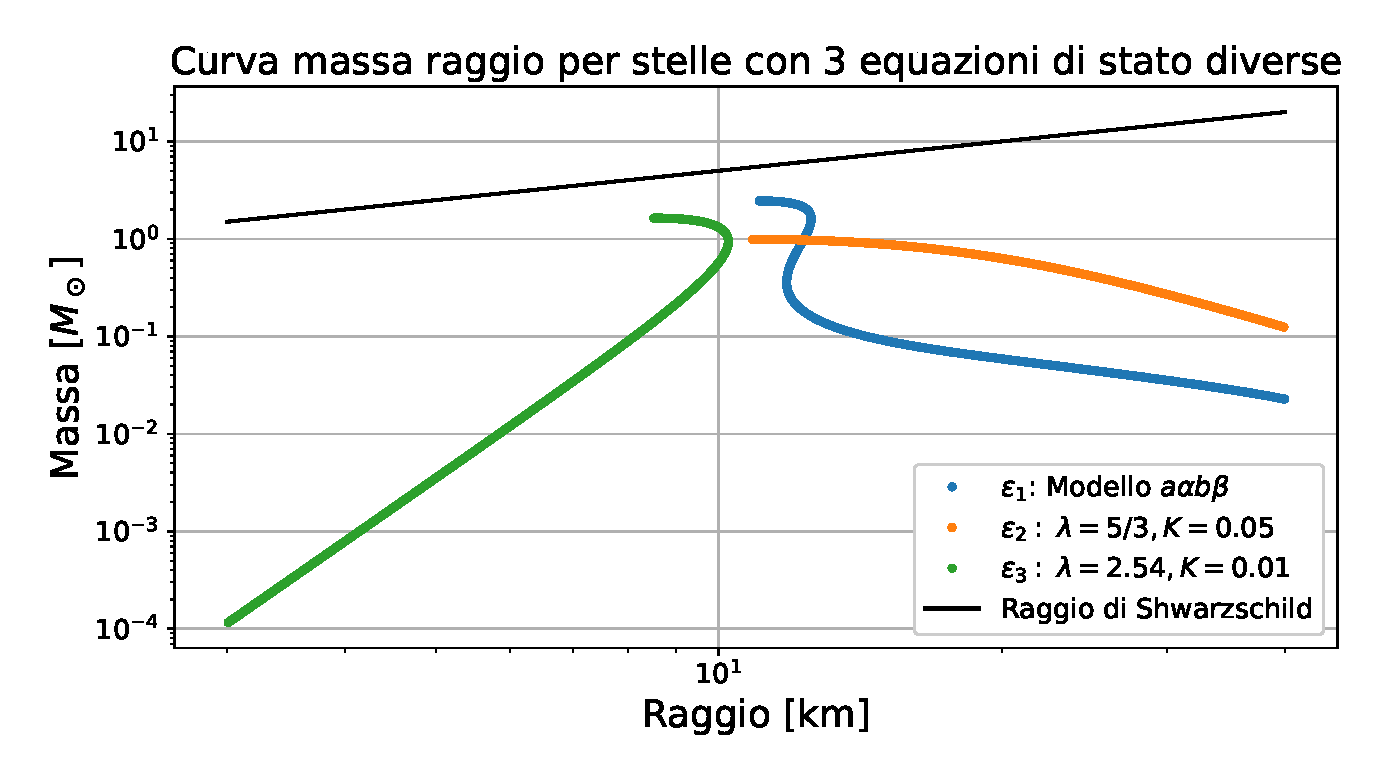
\includegraphics[width = 0.7 \textwidth]{Figures/MR.eps}
        \caption{Curva massa raggio per stelle di equzioni di stato
        $\epsilon_{1/2/3}$.
        La prima equazione di stato, quella più realistica,
        prevede stelle di neutroni più massive.}
        \label{fig:MR}
\end{figure}

Durante l'esecuzione del programma abbiamo inoltre smesso di incrementare la
pressione centrale iniziale quando la condizione di stabilità $\dv[]{M}{r} > 0$
veniva meno.

Notiamo subito che con l'equazione di stato \ref{eq:energia1} il modello prevede
stelle con massa e raggio maggiore rispetto al limite previsto dagli altri
modelli.

I valori della stella più massiva per ognuna delle 3 equazioni di stato vengono
riportati nella tabella \ref{tab:Mgrosso}.

\begin{table}[h!]
    \centering
    \begin{tabular}{c|c|c|c}
        & $P_0~[\Punit]$ & $R~[\unit{\kilo\meter}]$ & $M~[M_\odot]$ \\
         \hline
         $\epsilon_1$ & 885.2114 & 11.04289 & 2.456841 \\
         \hline
         $\epsilon_2$ & 217.2936 & 10.86752 & 0.990100 \\
         \hline
         $\epsilon_3$ & 948.5211 & 8.531525 & 1.635845 \\
    \end{tabular}
    \caption{Valori della pressione iniziale $P_0$, massa totale $M$ e raggio
    $R$ della stella più massiva per ogni equazione di stato utilizzata.}
    \label{tab:Mgrosso}
\end{table}


\section{Potenziale gravitazionale}

Come mostrato nel sistema \ref{eq:sistema_corr}, l'equzione che determina il
potenziale gravitazionale è disaccoppiata dalle altre due e, per $r \geq R$,
può anche essere risolta analiticamente.
Utilizzando le equazioni \ref{eq:Phi_ad} e \ref{eq:Phi_ext} possiamo trovare
l'espressione generale per il potenziale all'interno della stella riportata in
eq. \ref{eq:Phi_int1}.

\begin{equation}
    \Phi_\text{int} (\hat r) =
    \Phi_\text{ext} (\hat R) - \int_{\hat r}^{\hat R} \dv[]{\Phi}{x} \;\mathrm{d}x =
    \frac{1}{2} \log(1 - \frac{2 \hat M}{\hat R})
    + \int_{\hat r}^{\hat R} \frac{1}{\hat P (x) + \hat \epsilon (x)} \dv[]{\hat P (x)}{x} \;\mathrm{d}x
    \label{eq:Phi_int1}
\end{equation}

dove siamo stati attenti a rendere $\Phi (r)$ continuo per ogni $r \geq 0$
usando il valore di $\Phi_\text{ext}$ in $\hat R$. Infine sostituendo alla
derivata della pressione l'espressione in \ref{eq:P_ad} otteniamo

\begin{equation}
    \Phi_\text{int} (\hat r) =
    \frac{1}{2} \log(1 - \frac{2 \hat{M}}{\hat R}) + \int_{\hat r}^{\hat R}
    \frac{\hat m (x) + x^3 \hat P (x)}{2 \hat m (x) x - x^2}  \;\mathrm{d}x
    \label{eq:Phi_int2}
\end{equation}

Dati i valori di $\hat P (\hat r)$ e $\hat m (\hat r)$ che si ottengono
risolvendo le equazioni di stabilità possiamo quindi risolvere l'integrale con
il metodo dei trapezi per ottenere il valore di $Phi$ a ogni $r$ (Appendice
\ref{ap:Phi}).
Il grafico del potenziale gravitazionale ottenuto è mostrato in figura
\ref{fig:Phi}.

\begin{figure}[h!]
    \centering
    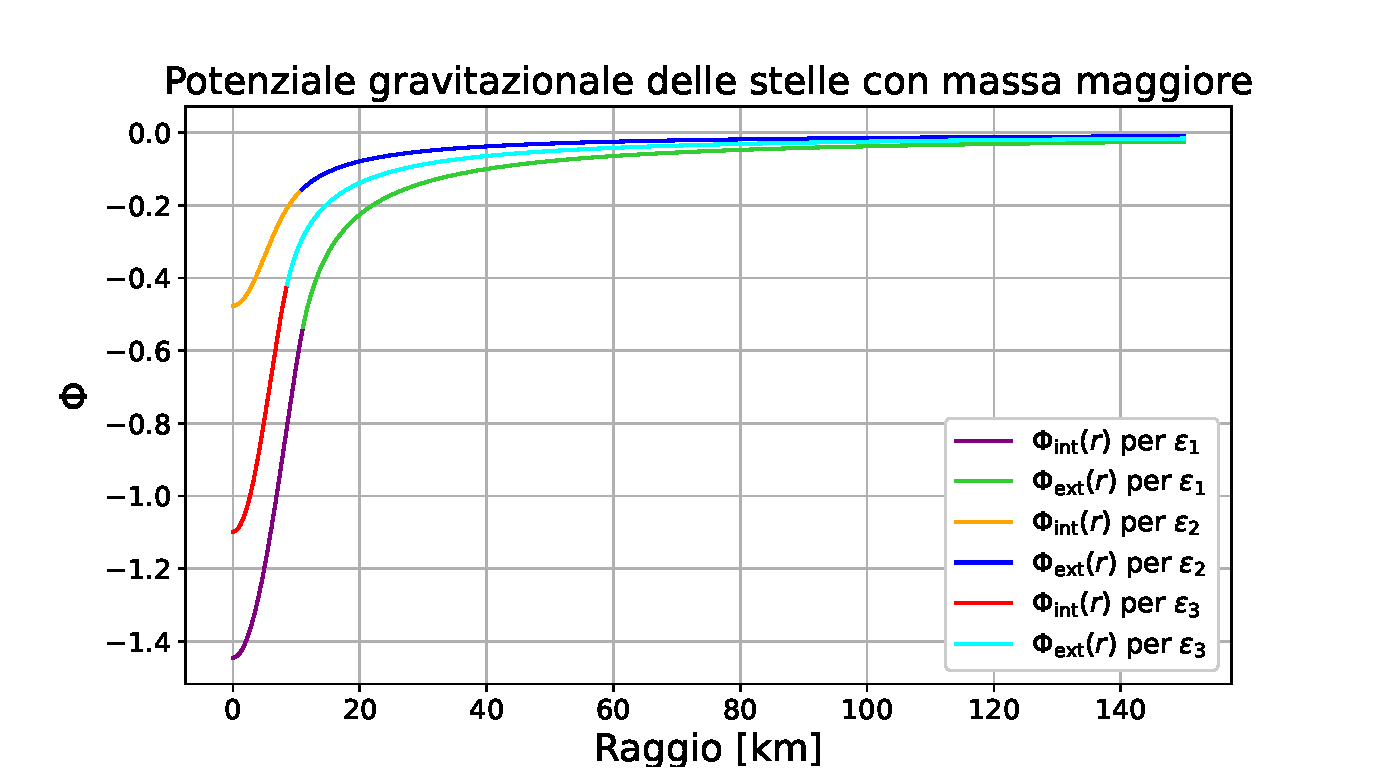
\includegraphics[width = 0.8 \textwidth]{Figures/Phi.eps}
    \caption{Grafico del potenziale gravitazionale all'interno e all'esterno
    della stella.
    Per $r < R$ è stato ottenuto integrando con il metodo dei trapezi l'eq.
    \ref{eq:Phi_int2}, per $r \geq R$ è stata plottata l'eq. \ref{eq:Phi_ext}}
    \label{fig:Phi}
\end{figure}

Vediamo dalla figura \ref{fig:Phi} che in tutti e 3 i casi $\Phi (r)$ è
continuo, grazie alla condizione imposta.

Il potenziale $\Phi$ (che fa parte del termine $e^{\Phi (r)} c^2 \mathrm{d}t^2$
della metrica $\mathrm{d}s^2$, che descrive la geometria dello spazio vicino
alla stella) assume un andamento famigliare: raggiunge valori più bassi per le
stelle più massive al diminuire di $r$ e tende a 0 per $r$ grandi.


\section{Radianza} \label{sec:rad}

In metrica di \Sh un fotone emesso a distanza $r$ con frequenza $\nu_\text{em}$
viene ricevuto da un osservatore a distanza $r'$ con una frequeza
$\nu_\text{ric}$ data da

\begin{equation}
    \frac{\nu_\text{ric}}{\nu_\text{em}} = e^{\Phi (r) - \Phi (r')} \, .
\label{eq:redshift}
\end{equation}

Dove $\Phi (r)$ è propio il potenziale gravitazionale mostrato in figura
\ref{fig:Phi}.

La radianza di una stella si può esprimere con l'equazione di Plank per il corpo
nero

\begin{equation}
    B(\nu, T) = \frac{2 h \nu ^3}{c^2} \frac{1}{e^{h \nu / (k_B T)} - 1}
    \label{eq:rad}
\end{equation}

dove $T$ è la temperatura della stella e $h$ la costante di Plank.
Per fare i conti considerando solo il caso con $K_B T = 1
\unit{\mega\electronvolt}$ e mettiamo l'equzione \ref{eq:rad} in funzione di
variabili adimensionali. Otteniamo

\begin{equation}
    \hat B(\hat \nu) = \frac{\hat \nu ^3 }{e^{\hat \nu} - 1}
    \label{eq:B_ad}
\end{equation}
dove abbiamo definito
\begin{align}
    \nu_0 &= \frac{\nu}{\hat \nu} = \frac{1\unit{\mega\electronvolt}}{h} \simeq
    \num{2.417989e20} \unit{\hertz} \label{eq:B0def}\\
    B_0 &= \frac{B}{\hat B} = \frac{2 h \nu_0^3}{c^2}
    = \frac{2 \unit{\mega\electronvolt}}{(h c)^2} \simeq \num{1.301059e-6}
    \frac{\unit{\mega\electronvolt}}{\unit{\femto\meter\squared}}
    \label{eq:nu0def}
\end{align}

Infine, se consideriamo l'effetto doppler dovuto al potenziale gravitazionale
descritto in eq. \ref{eq:redshift} e utilizziamo la formula analitica per il
potenziale gravitazionale all'esterno della stella (eq. \ref{eq:Phi_ext}),
otteniamo

\begin{equation}
    \hat \nu_\text{em} = \hat \nu_\text{ric}
    \left ( \frac{1 - \frac{2 \hat M}{r}}{1 - \frac{2 \hat M}{\hat R}}\right )^{1/2}
    \quad
    \implies
    \quad
    \hat B(\hat \nu_\text{ric}, \hat r) =
    \frac{\hat \nu_\text{ric}^3 \left(1 - \frac{2 \hat M}{\hat r}\right)^{3/2}
    \left(1 - \frac{2 \hat M}{\hat R}\right)^{-3/2} }
    {\exp( \hat \nu_\text{ric} \left(1 - \frac{2 \hat M}{\hat r} \right)^{1/2}
    \left(1 - \frac{2 \hat M}{\hat R}\right)^{-1/2} ) - 1}
    \label{eq:B_corr}
\end{equation}

Nel figure \ref{fig:rad1}, \ref{fig:rad2} e \ref{fig:rad3} viene studiato lo
spettro della radiazione emessa per le 3 stelle massive di cui abbiamo studiato
il potenziale in \ref{fig:Phi} a distanze diverse dalla stella.
In blu è plottata l'eq. \ref{eq:rad}, ovvero la radianza senza correzioni
relativistiche.

\begin{figure}[h]
    \begin{minipage}{0.49\textwidth}
        \centering
        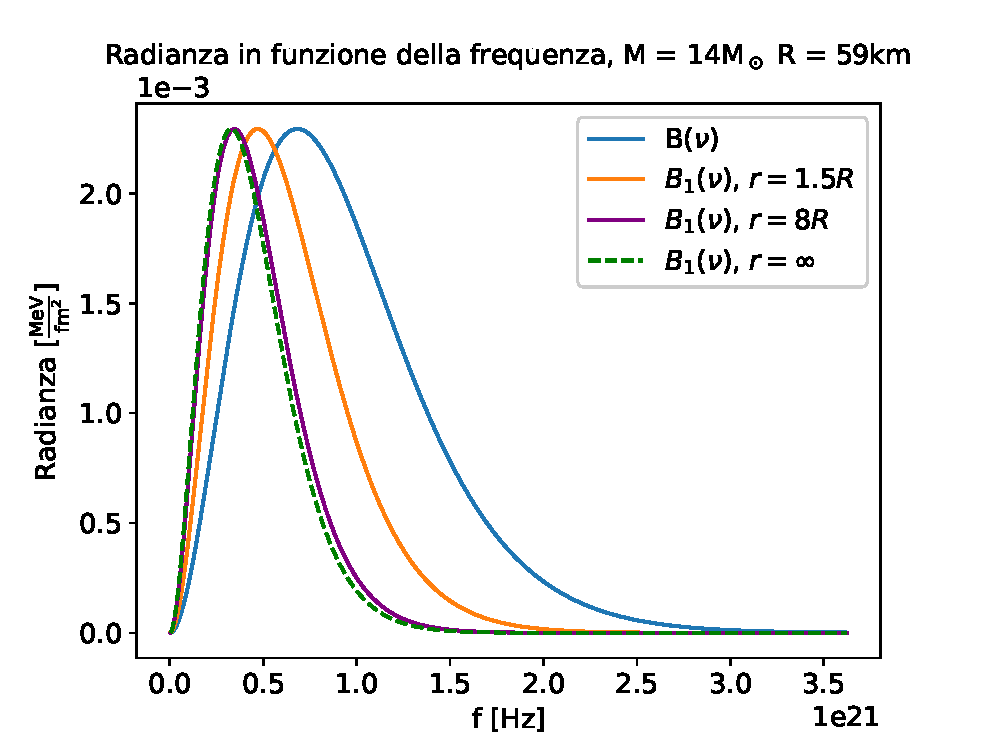
\includegraphics[width = \textwidth]{Figures/radianza1.eps}
        \caption{Radianza di una stella con $M = 2.5M_\odot$ e
        $R = 11.0\unit{\kilo\meter}$, percepita a $16.5 \unit{\kilo\meter}$,
        $88 \unit{\kilo\meter}$ e a distanza infinita.
        Essendo la stella con massa maggiore è anche quella in cui la curva è
        più spostata verso sinistra.}
        \label{fig:rad1}
    \end{minipage}
    \hspace{0.015\textwidth}    
    \begin{minipage}{0.49\textwidth}
        \centering
        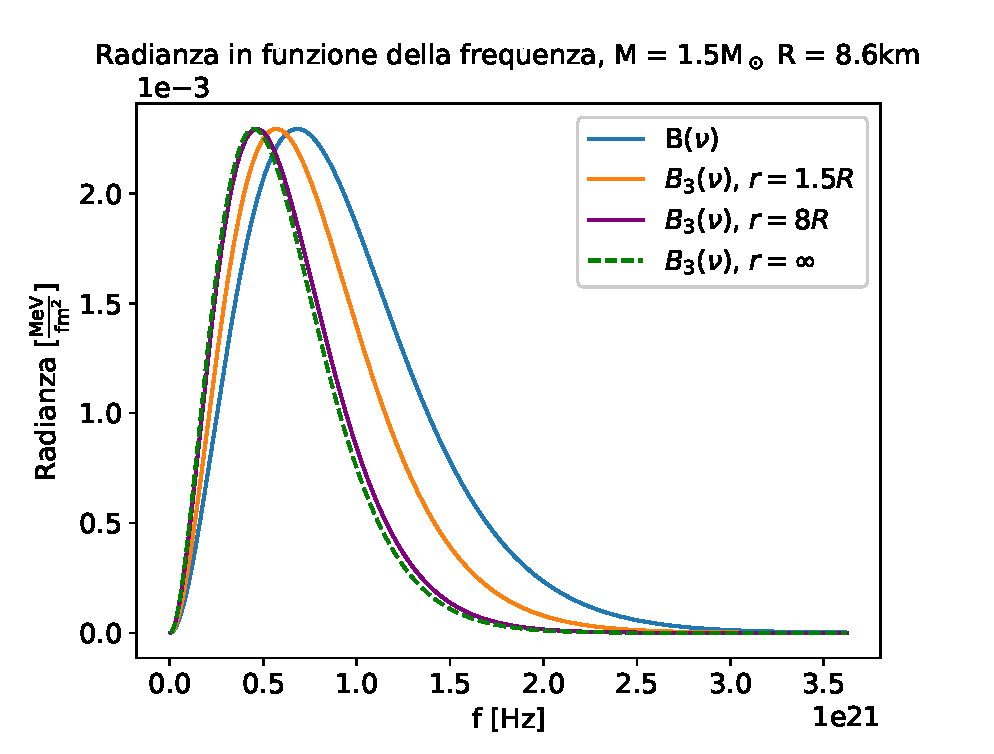
\includegraphics[width = \textwidth]{Figures/radianza3.eps}
        \caption{Radianza da una stella con $M = 1.6M_\odot$ e
        $R = 8.5\unit{\kilo\meter}$, percepita a $12.8 \unit{\kilo\meter}$,
        $68 \unit{\kilo\meter}$ e a distanza infinita.
        In blu la radianza senza correzioni relativistiche.\\}
        \label{fig:rad2}
    \end{minipage}
\end{figure}

La curva in tutti e 3 i casi subisce uno spostamento verso le frequenze più
basse, \textit{redshift} per l'appunto, e l'effetto è tanto maggiore quanto più
la stella è massiva e l'osservatore distante. Già a una distanza di 8 volte il
raggio della stella la curva della radianza è molto simile a quella
all'inifinito, in cui il termine $\Phi (r')$ in eq. \ref{eq:redshift} è
trascurabile.
\begin{figure}[h]
    \centering
    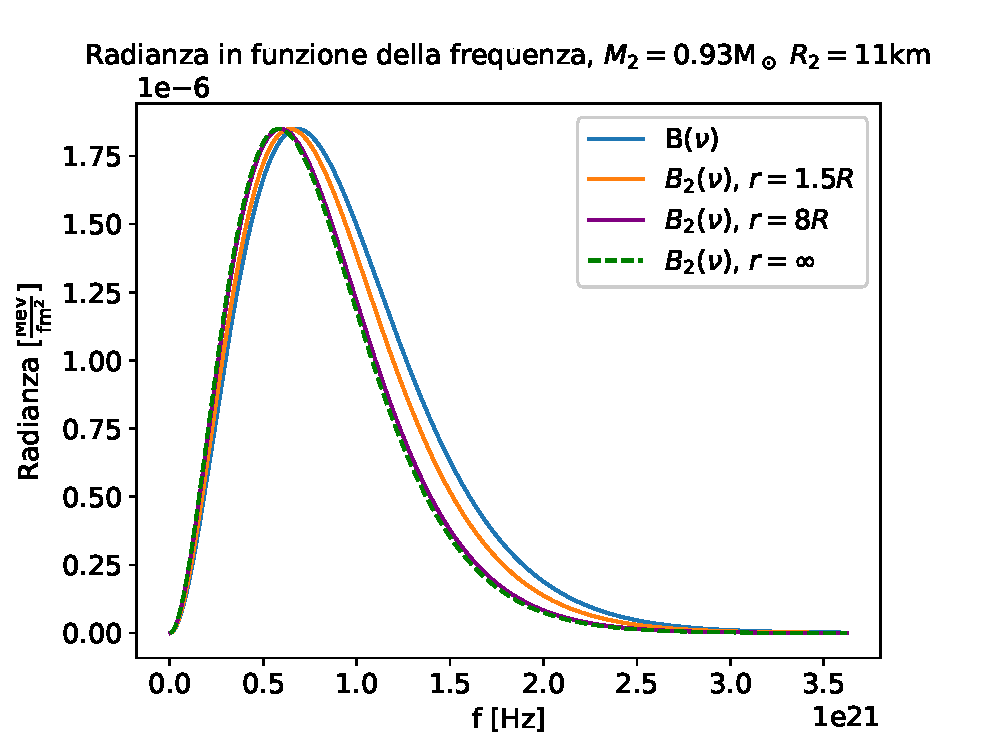
\includegraphics[width = 0.6 \textwidth]{Figures/radianza2.eps}
    \caption{Radianza da una stella con $M = 0.99M_\odot$ e
    $R = 10.8\unit{\kilo\meter}$, percepita a 16.2, 86.4 \unit{\kilo\meter} e a
    distanza infinita.
    In blu la radianza senza correzioni relativistiche.}
    \label{fig:rad3}
\end{figure}


\section{Potenza emessa}
La potenza totale emessa dalla stella per un elemento della sua superficie, si
può ottenere integrando la radianza $B(\nu, T)$ sulle frequenze e sull'angolo
solido, con l'accortezza di moltiplicare per un fattore $\cos(\theta)$ (Legge
di Lambert) per proiettare la radiazione lungo la normale alla superficie
sottesa da $\mathrm{d}\Omega$.

\begin{align}
    \mathcal P &= \int_0^\infty \mathrm{d}\nu \int B(\nu, T) \cos(\theta) \;
    \mathrm{d}\Omega
    =  \int_0^{A k_B T} B(\nu, T) \; \mathrm{d}\nu ~ 
    \int_0^{2 \pi} \mathrm{d}\phi \int_0^1 \mathrm{d}(\cos(\theta)) \;
    \cos(\theta) \\
    &\simeq \pi \int_{\nu_\text{ric} = 0}^{\nu_\text{ric}
    = A k_B T} B(\nu_\text{em}, T) \; \mathrm{d}\nu_\text{ric}
    \label{eq:Pot}
\end{align}

Nell'ultimo passaggio (eq. \ref{eq:Pot}) è esplicitato che l'integrazione viene
fatta su $\nu_\text{ric}$, ovvero le frequenze misurate a distanza r, abbiamo
messo un upperbound finito all'integrale e, per semplificare i calcoli per il
prossimo punto, abbiamo lasciato la dipendenza da $\nu_\text{em}$ in $B$.

Passiamo quindi alle unità adimensionali, riportate in eq. \ref{eq:PT_ad}, e
facciamo un cambio di variabile all'interno dell'integrale utilizzando la
formula del redshift $\nu_\text{ric} = \nu_\text{em} e^{\Phi(R) - \Phi(r)}$:

\begin{align}
    \hat{\mathcal P}(\hat r)
    &= \int_{\hat \nu_\text{ric} = 0}^{\hat \nu_\text{ric} = \frac{A T_0}{\nu_0}}
    \hat B (\hat \nu_\text{em}, \hat T) \; \mathrm{d} \hat \nu_\text{ric}
    = e^{\Phi(\hat R) - \Phi(\hat r)}
    \int_{\hat \nu_\text{em} = 0}^{\hat \nu_\text{em} = \frac{A T_0 \hat T}{\nu_0} e^{\Phi(\hat R) - \Phi(\hat r)}}
    \frac{\hat \nu_{em}^3}{\exp(\hat \nu_\text{em} / \hat T) - 1} \; \mathrm{d}\hat \nu_\text{em} \\
    &= \left(1 - \frac{2 \hat M}{\hat R} \right)^{1/2}
    \left(1 - \frac{2 \hat M}{\hat r} \right)^{-1/2}
    \int_0^{\frac{A T_0 \hat T}{\nu_0} e^{\Phi(\hat R) - \Phi(\hat r)}}
    \frac{\nu^3}{e^{\nu / \hat T} - 1} \; \mathrm{d} \nu \\
    &= \left(1 - \frac{2 \hat M}{\hat R} \right)^{1/2}
    \left(1 - \frac{2 \hat M}{\hat r} \right)^{-1/2}
    \int_0^{\frac{A T_0 \hat T}{\nu_0}} \frac{\nu^3}{e^{\nu / \hat T} - 1} \;
    \mathrm{d} \nu \, .
    \label{eq:Pot_ad}
\end{align}

Dove sono state usate le definizioni di $B(\hat \nu, \hat T)$ (eq.
\ref{eq:B_ad}) e quella di $\Phi (r)$ (eq. \ref{eq:Phi_ext}) e nell'ultimo
passaggio in \ref{eq:Pot_ad} si è utilizzato il fatto che nell'integrale
$A \to \infty$ e che $e^{\Phi(R) - \Phi(r)} < 1$, ignorare il termine migliora
quindi la nostra approssimazione.

\begin{equation}
    \mathcal P_0 = \frac{\mathcal P}{\hat {\mathcal P}}
    = \pi B_0 \nu_0 \simeq \num{9.883290e+14} \,
    \frac{\unit{\mega\electronvolt}}{\unit{\second\femto\meter\squared}} \, ,
    \quad \quad
    T_0 = T / \hat T = 1 \unit{\mega\electronvolt} \, .
    \label{eq:PT_ad}
\end{equation}


\subsection{Convergenza dell'integrale}
Dal momento che numericamente non è possibile integrare sulle frequenze fino a
$\nu = + \infty$, nei passaggi in eq. \ref{eq:Pot} e poi in eq. \ref{eq:Pot_ad}
abbiamo utilizzato un parametro $A$ che deve essere sufficientemente grande da
poter approssimare in modo ragionevole l'integrale, per i valori di $\hat T$
utili.
Riportiamo in eq. \ref{eq:integrale} l'integrale da calcolare.

\begin{equation}
    \mathcal{I} (\hat T) = \int_0^{\frac{A T_0 \hat T}{\nu_0}} \frac{\nu^3}{e^{\nu / \hat T} - 1} \; \mathrm{d} \nu 
    = \int_0^{\frac{A T_0}{\nu_0}} \frac{\nu^3}{e^{\nu / \hat T} - 1} \; \mathrm{d} \nu \, .
    \label{eq:integrale}
\end{equation}

A priori gli estremi di integrazione dipendono da $\hat T$, dal momento che stiamo studiando la radiazione emessa da stelle di neutroni siamo interessati a studiare un range di temperature più piccolo.
In particolare non di troppo superiori a $k_B T = 1 \unit{\mega\electronvolt}$, ovvero $\hat T = 1$ che decidiamo essere il nostro upperbound per la temperatura.
Per temperature inferiori la funzione va a 0 più velocemente e quindi l'approssimazione di $A$ come finito è ancora migliore.

Facendo riferimento alla figura \ref{fig:rad2} dove in blu è plottata la funzione che dobbiamo integrare per $\hat T = 1$, possiamo vedere che per $\nu > \num{3.5e21} \unit{\hertz}$ la radianza è quasi nulla.
In quell'occasione era stata calcolata $\hat B(\hat \nu)$ con $\hat \nu$ tra $0$ e $15$. Come stima iniziale possiamo quindi integrare fino a $\hat \nu = 20$ che corrisponde a

\begin{equation}
    \frac{A \, T_0}{\nu_0} = 20
    \quad \iff \quad
    A = 20 \, \frac{\nu_0}{T_0} \simeq \num{4.835978e21} \, \unit{\per\mega\electronvolt\per\second}
    \label{eq:A}
\end{equation}

Possiamo ottenere un valore migliore valutando la convergenza dell'integrale.

Per prima cosa verifichiamo per quale \texttt{N} (numero di step nell'integrazione) il valore di $\mathcal{I}$ converge (il codice si trova in Appendice \ref{ap:integrali}).
In questo caso la situazione peggiore è quella per temperature molto piccole, scegliamo come lowerbound $\hat T = 0.01$, poiché la curva è molto piccola e stretta.
Otteniamo il grafico in figura \ref{fig:Pot_cvgN}.
I valori sono degli scarti rispetto a $\mathcal{I}_{N = 1e8}$ (l'integrale calcolato con $N = \num{1e8}$) e sono normalizzati rispetto allo stesso.
Al contriario di quello che succede di solito, il metodo Simpson (che ha un costo computazionale maggiore), non presenta vantaggi rispetto a quello dei trapezi.
Dal codice (Appendice \ref{ap:integrali}) che genera i dati mostrati in figura \ref{fig:Pot_cvgN} otteniamo un errore relativo minore di $\num{1e-7}$ per \texttt{N\_trap = 19060} e \texttt{N\_simp = 25368}.
\begin{figure}[h]
    \begin{minipage}{0.49 \textwidth}
        \centering
        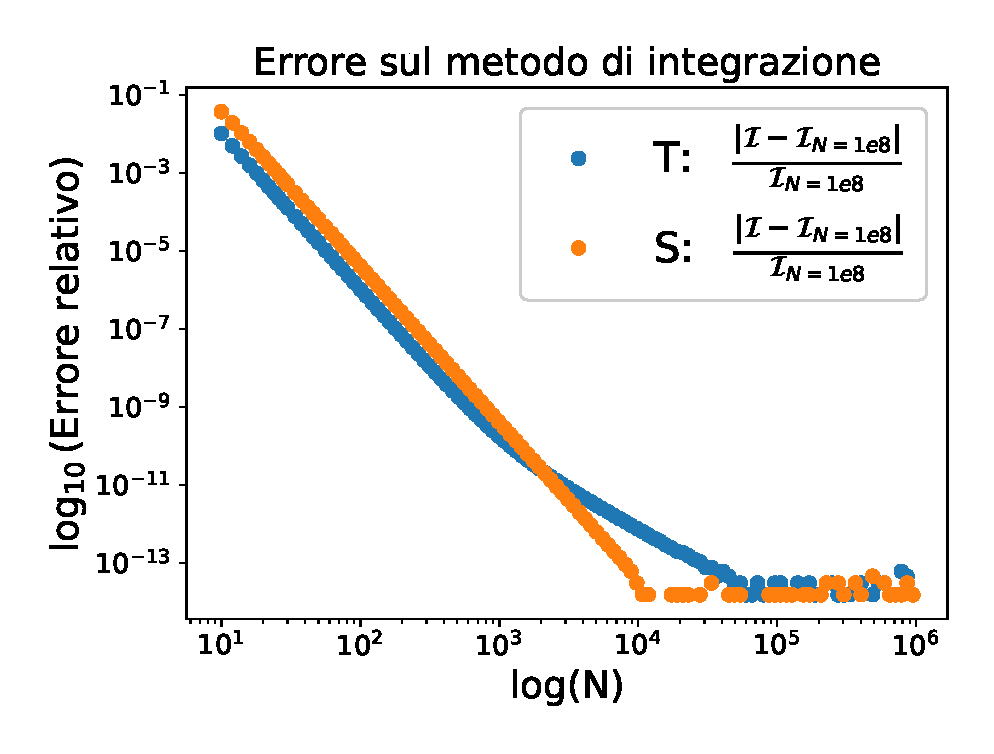
\includegraphics[width = \textwidth]{Figures/Pot_cvgN.eps}
        \caption{Errore relativo sul calcolo di $\mathcal I(1)$ per diversi \texttt{N} (numero di step nell'integrazione con i trapezi, \textbf{T}, e con simpson, \textbf{S}).  \\ \\}
        \label{fig:Pot_cvgN}
    \end{minipage}
    \hspace{0.01 \textwidth}
    \begin{minipage}{0.49 \textwidth}
        \centering
        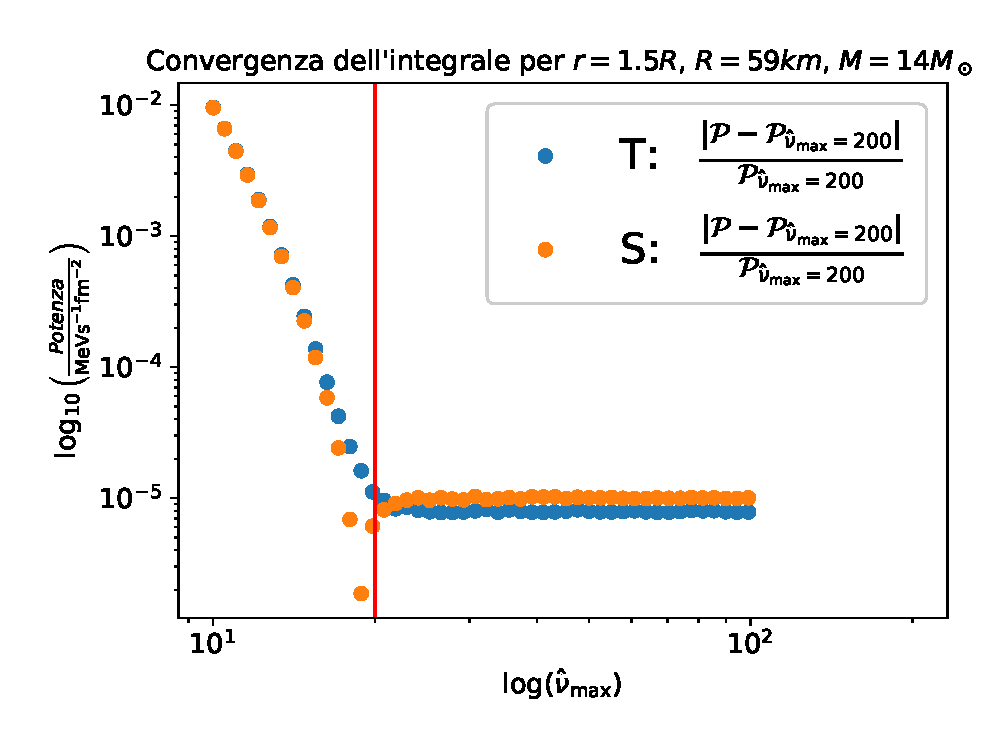
\includegraphics[width = \textwidth]{Figures/Pot_cvgA.eps}
        \caption{Errore relativo sul calcolo di $\mathcal I (1)$ per diversi valori di $\hat \nu_\text{max}$.
        Poco dopo la stima iniziale di  $\hat \nu_\text{max} = \num{20}$ (line verticale rossa) l'errore si stabilizza.
        L'errore non diminuisce come prima perché c'è una sorta di offset dato dall'aver fissato il rapporto \texttt{N / nu\_max}.}
        \label{fig:Pot_cvgA}
    \end{minipage}
\end{figure}

Fissati \texttt{N\_trap} e \texttt{N\_simp} per un intervallo $\Delta \hat \nu = 20$ proponiamo quindi in figura \ref{fig:Pot_cvgA} lo stesso tipo di grafico degli scarti fatto però in funzione della scelta di $\nu_\text{max}$, dove abbiamo tenuto costante il valore \texttt{N / nu\_max} apena ottenuto.
Questa volta si studia il caso in cui $r = R_1$, ovvero quello in cui la curva è più spostata verso destra e serve un upper bound maggiore.

Dallo script per generare i dati mostrati in figura \ref{fig:Pot_cvgA} otteniamo un errore di $\num{1e-7}$ per

\begin{table}[h]
    \centering
    \begin{tabular}{ccc}
         & N & $\hat \nu_\text{max}$ \\
        \hline
        Trapezi & 22936 & 24.0661923 \\
        \hline
        Simpson & 30516 & 24.0661923 \\
    \end{tabular}
\end{table}

Di conseguenza possiamo valutare

\begin{equation}
    A = 24.0661923 \, \nu_0 \, \unit{\per\mega\electronvolt} \simeq \num{5.819179e21} \, \unit{\per\mega\electronvolt\per\second}
    \label{eq:A_giusto}
\end{equation}

Con questi parametri otteniamo i valori $\mathcal I_T$, per i trapezi, e $\mathcal I_S$, per Simpson:

\begin{equation}
    \mathcal I_T (1) = 6.4939388
    \quad \quad \quad
    \mathcal I_S (1) = 6.4939388 \, .
    \label{eq:val_I}
\end{equation}

Gli integrali hanno lo stesso valore poiché ci siamo assicurati di avere una
precisione di $\num{1e-7}$ per il caso perggiore a $\hat T = 0.01$, che servirà
nella sezione \ref{sec:temp_perc}.


\subsection{Potenza totale in funzione della distanza}

Studiato l'integrale che serve per il calcolo della potenza possiamo riscrivere $\mathcal{\hat P}$ così

\begin{equation}
    \mathcal{\hat P} (\hat r, \hat T) = \left(1 - \frac{2 \hat M}{\hat R} \right)^{1/2} \left(1 - \frac{2 \hat M}{\hat r} \right)^{-1/2} \mathcal I (\hat T)
    \label{eq:Pot_I}
\end{equation}

Riportiamo quindi in figura \ref{fig:Pot} il l'andamento di $\mathcal P (r, \hat T = 1)$ per le stelle più massive descritte in \ref{tab:Mgrosso}.

\begin{figure}[h]
    \centering
    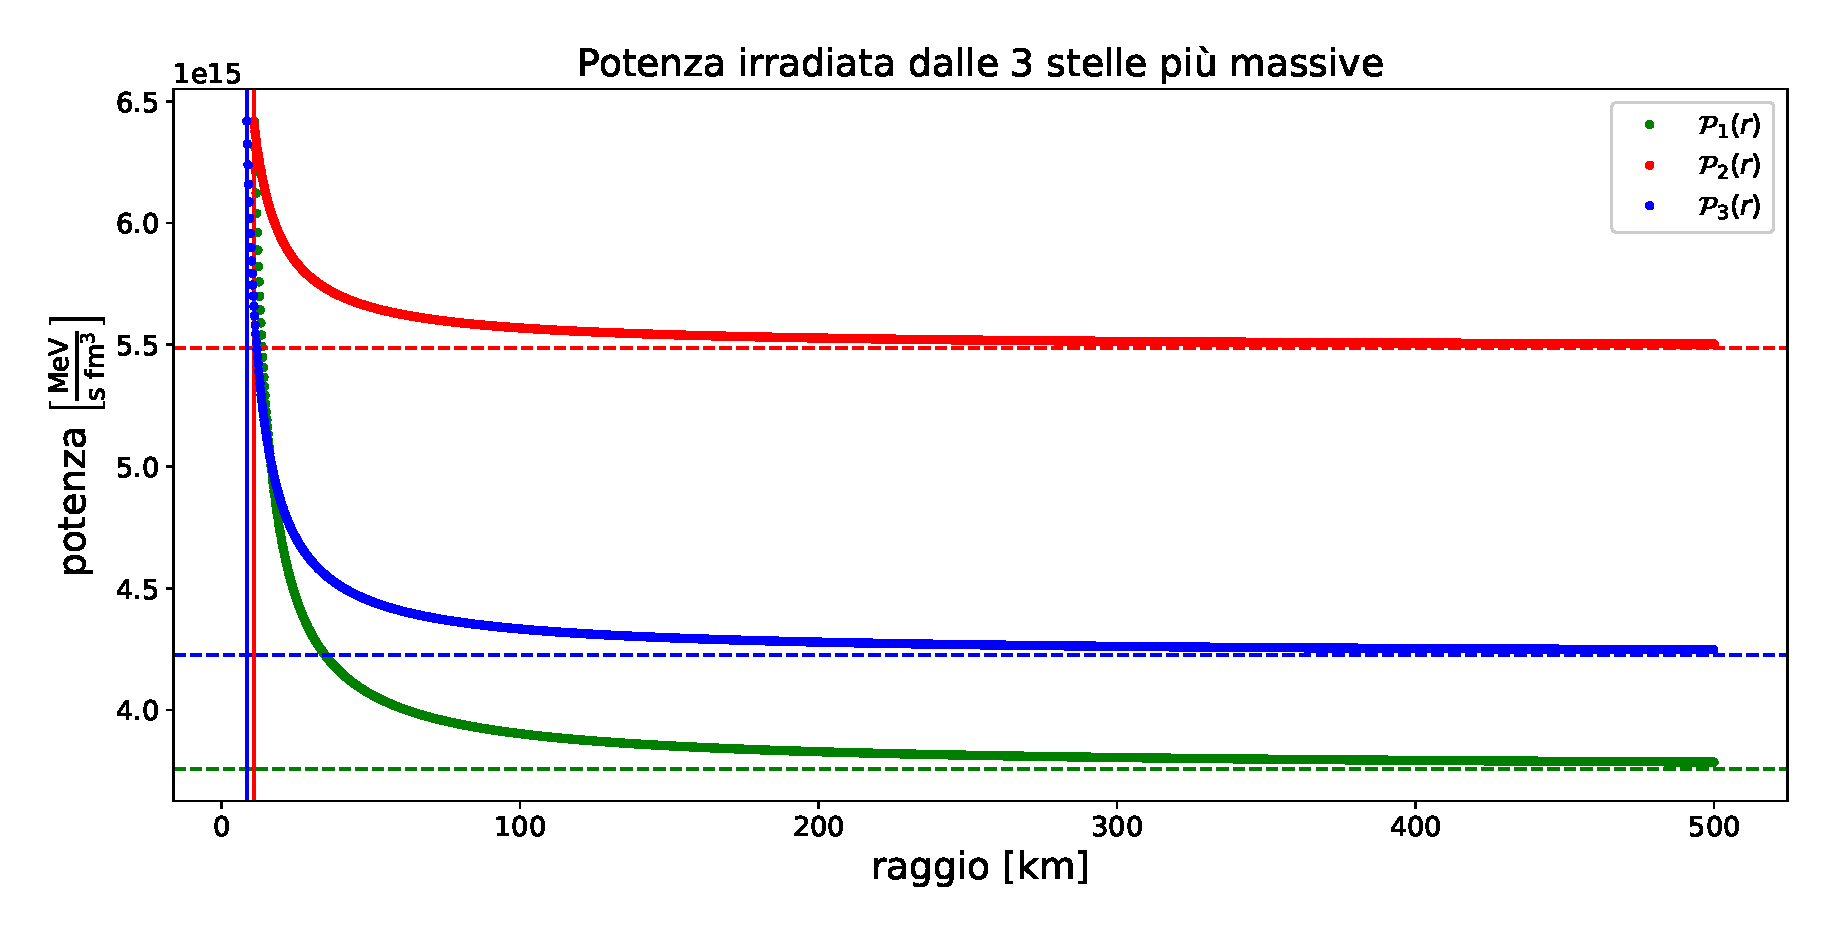
\includegraphics[width = \textwidth]{Figures/Pot.eps}
    \caption{Potenza in funzione della distanza per le 3 stelle: $(R_1 = 59.0 \unit{\kilo\meter},~M_1 = 14.3 M_\odot)$, $(R_2 = 10.9 \unit{\kilo\meter},~M_2 = 0.926 M_\odot)$ e $(R_3 = 8.56 \unit{\kilo\meter},~M_3 = 1.53 M_\odot)$.
    La linea continua verticale rappresenta il raggio della stella, la linea tratteggiata orizzontate il valore di $\mathcal{P}$ a $r = \infty$.}
    \label{fig:Pot}
\end{figure}

Con linea tratteggiata e linea continua sono rispettivamente rappresentati raggio e valore della potenza all'infinito per ogni stella analizzata.



\newpage


\section{Temperatura Percepita}
\label{sec:temp_perc}

Una volta ottenuta la potenza totale irradiata da una stella è possibile calcolare la sua temperatura, grazie alla relazione

\begin{equation}
    k_B T_{eff} = \left( \mathcal{P} (T) \frac{15 c^2 h^3}{2 \pi^5} \right)^{1/4}
    \label{eq:Teff}
\end{equation}

Dove $T_{eff}$ è la temperatura percepita a una certa distanza dalla stella e $T$ la temperatura reale, che si misurerebbe a $r = R$.

Mettendo le variabili adimensionali, sostituendo a $\mathcal{\hat P}$ l'espressione in \ref{eq:Pot_I} e ricordando le espressioni di $\mathcal{\hat P}_0$ (eq. \ref{eq:PT_ad}), $B_0$ (eq. \ref{eq:B0def}) $\nu_0$ (eq. \ref{eq:nu0def}) e che $T_0 = \unit{\mega\electronvolt}$, otteniamo

\begin{align}
    T_0 \hat T_{eff} &= \left( \mathcal P_0 \frac{15 c^2 h^3}{2 \pi^5} \right)^{1/4} \mathcal{\hat P}^{1/4}
    = \frac{15^{1/4}}{\pi} \unit{\mega\electronvolt} \left(1 - \frac{2 \hat M}{\hat R} \right)^{1/8} \left(1 - \frac{2 \hat M}{\hat r} \right)^{-1/8} \mathcal{I} (\hat T)^{1/4} \\
    \hat T_{eff}(\hat r, \hat T) &= \frac{15^{1/4}}{\pi} \left(1 - \frac{2 \hat M}{\hat R} \right)^{1/8} \left(1 - \frac{2 \hat M}{\hat r} \right)^{-1/8} \mathcal{I} (\hat T)^{1/4}
    \label{eq:Teff_ad}
\end{align}

Possiamo quindi studiare l'equzione \ref{eq:Teff_ad} per le 3 stelle studiate in precedenza, questa volta però fissiamo $r = \infty$ e studiamo la $T_{eff}$ in funzione di $T$, la temperatura propria della stella, facendo il limite

\begin{equation}
    \hat T_{eff}(\hat r, \hat T) = \frac{15^{1/4}}{\pi} \left(1 - \frac{2 \hat M}{\hat R} \right)^{1/8} \mathcal{I} (\hat T)^{1/4}
\end{equation}

Presentiamo il grafico in figura \ref{fig:Teff}, il codice si trova nell'appendice \ref{ap:Teff}.

\begin{figure}[h]
    \centering
    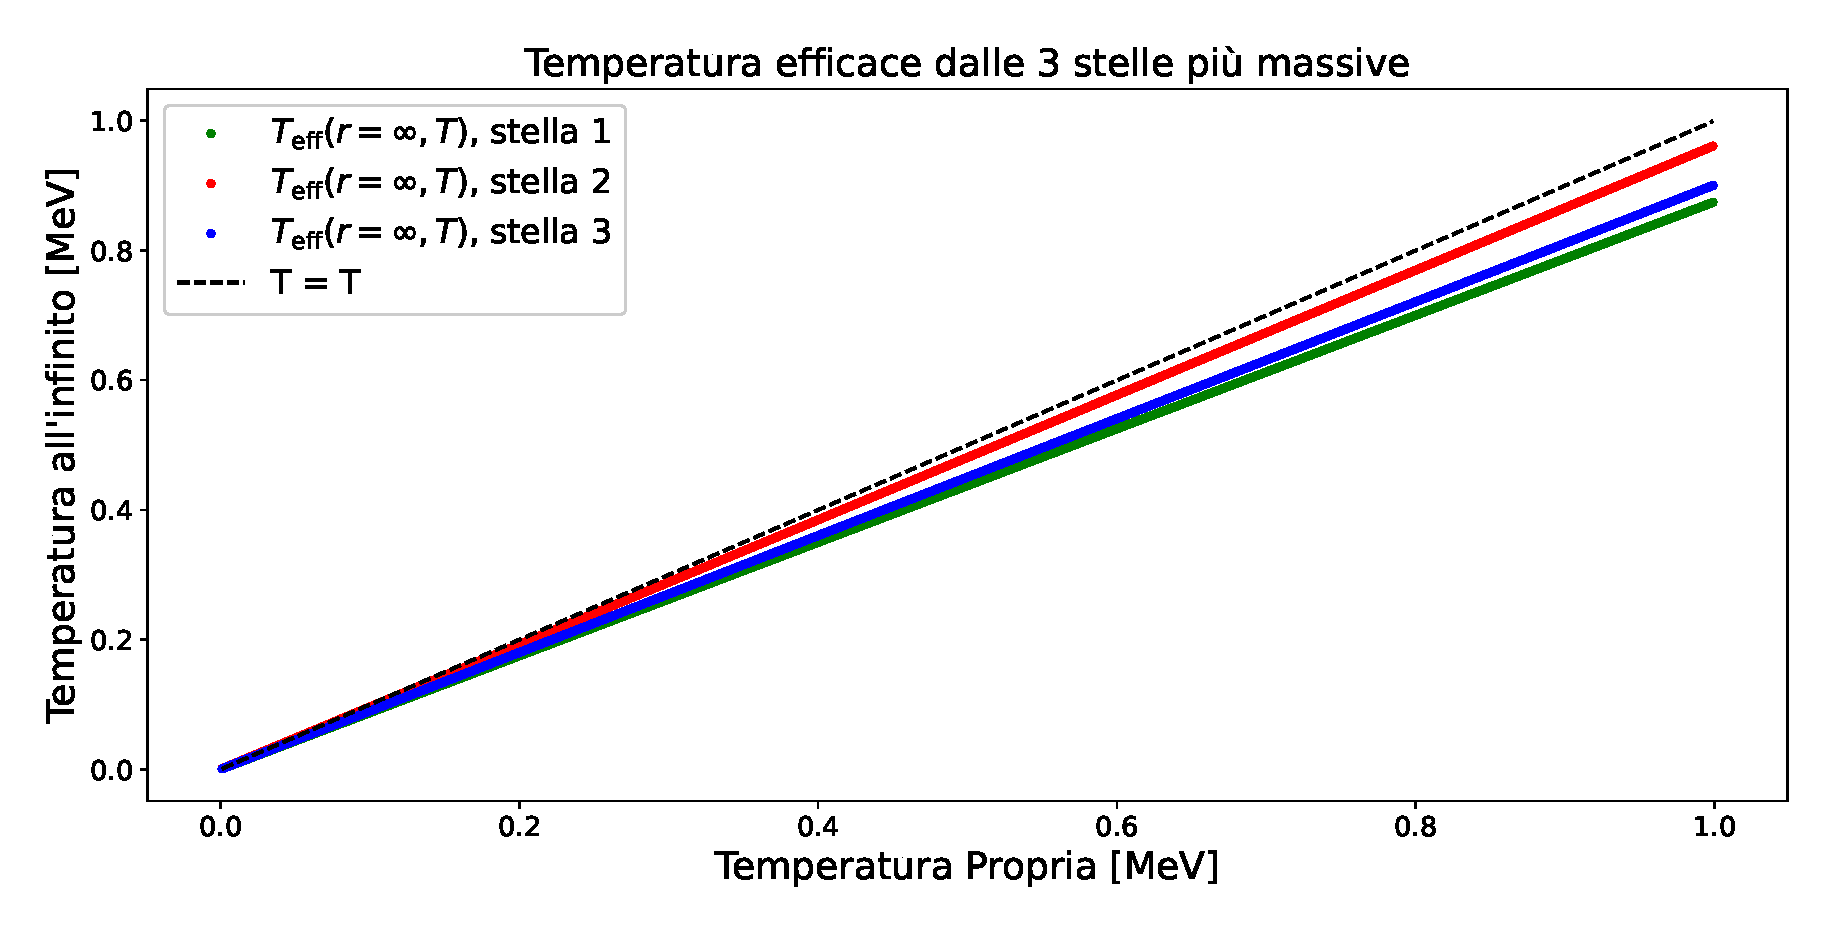
\includegraphics[width = \textwidth]{Figures/Teff.eps}
    \caption{Temperatura percepita all'infinito delle 3 stelle con masse $M_1 = 14.3 M_\odot$, $M_2 = 0.925 M_\odot$ e $M_3 = 1.53 M_\odot$. Come ci aspettavamo la temperatura misurata all'infinito è sempre minore di quella propria della stella.}
    \label{fig:Teff}
\end{figure}

Come ci aspettavamo la temperatura percepita all'infinito è sempre minore di quella propria della stella.
Il grafico mostra anche un'incidenza diversa del redshift per le 3 stelle.
In accordo con quello osservato in figura \ref{fig:Phi} e \ref{fig:Pot} i fotoni subiscono il redshift maggiore per la stella più massiva $M_1 = 14.3 M_\odot$ e seguono in ordine (sempre di massa) effetti minori per $M_3 = 1.53 M_\odot$ e $M_2 = 0.925 M_\odot$.


\section{Temperatura efficace in funzione della pressione centrale}

Si presentano in fine i grafici della temperatura efficacie in funzione della
pressione centrale della stella.
Vengono mostrati i grafici per tutti i 3 i tipi di politropico.
Viene inoltre mostrato sia il caso per la temperatura della stella
$\hat T = 1$ (Figura \ref{fig:Teff1_su_P} che quello per $\hat T = 0.01$
(Figura \ref{fig:Teff001_su_P}.
Come ci si poteva aspettare una pressione centrale maggiore porta a una stella
più massiva, il cui redshift gravitazionale è più forte.


\begin{figure}[h]
    \begin{minipage}{0.49 \textwidth}
        \centering
        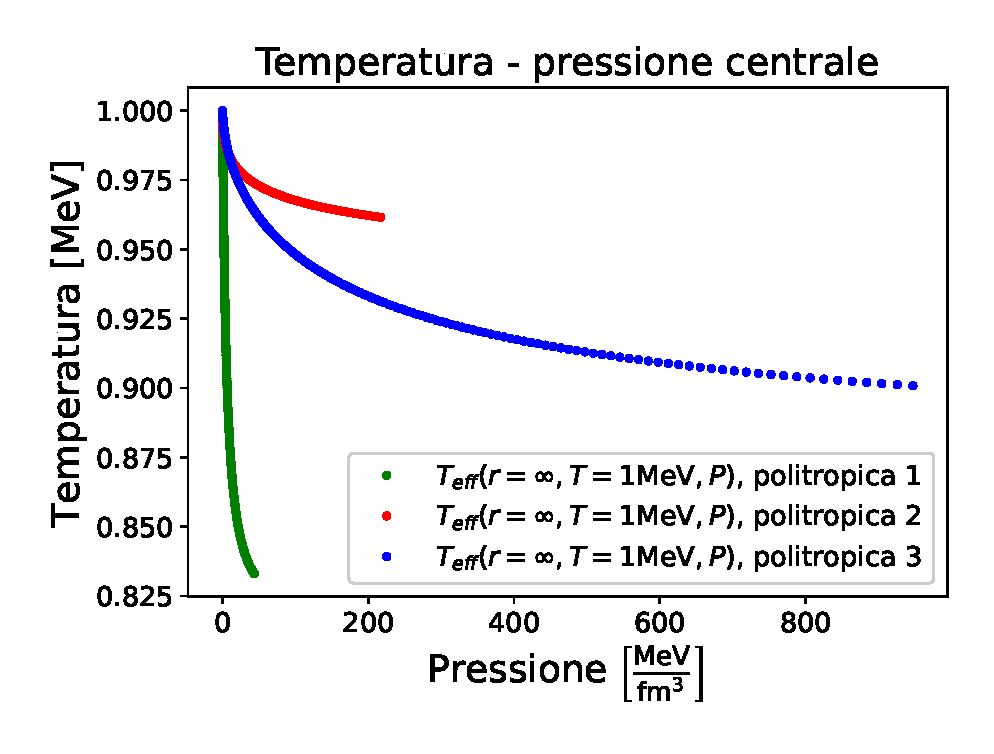
\includegraphics[width = \textwidth]{Figures/Teff1_su_P.eps}
        \label{fig:Teff1_su_P}
    \end{minipage}
    \hspace{0.015 \textwidth}
    \begin{minipage}{0.49 \textwidth}
        \centering
        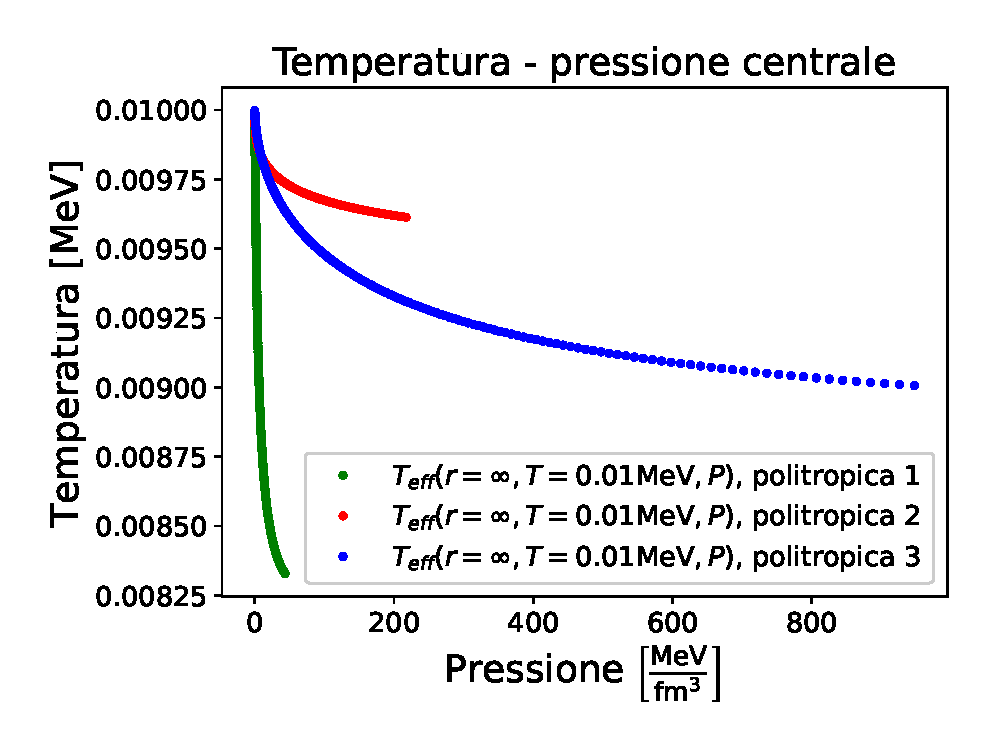
\includegraphics[width = \textwidth]{Figures/Teff001_su_P.eps}
        \label{fig:Teff001_su_P}
    \end{minipage}
    \caption{Fissata la temperatura della stella ($\hat T = 1$ a sinistra e
    $\hat T = 0.01$ a destra) è possibile utilizzare la temperatura misurata
    all'infinito come parametro per stimare la pressione centrale, data una
    politropica.}
\end{figure}















\newpage
\appendix


%%%%%%%%%%%%%%%%%%%%%%%%%%%%%%%%%%%%%%%%%%%%%%%%%%%%%%%%%%%%%%%%%%%%%%%%%%%%%%%%
%%%%%%%%%%%%%%%%%%%%                APPENDICI               %%%%%%%%%%%%%%%%%%%% 
%%%%%%%%%%%%%%%%%%%%%%%%%%%%%%%%%%%%%%%%%%%%%%%%%%%%%%%%%%%%%%%%%%%%%%%%%%%%%%%%


\section{RK4} \label{ap:RK4}
Codice con cui è stato implementato il metodo \texttt{RK4}. \texttt{fun\_P()} e \texttt{fun\_m()} sono le funzioni presenti a destra dell'uguale nella prima e nella seconda riga del sistema \ref{eq:sistema_adim}.

\begin{lstlisting}[language=C]
void rungeKutta4(double h, double r, double *P, double *m, int tipo_politropica){

    double k1, k2, k3, k4, l1, l2, l3, l4;

    k1 = h * fun_m(r, *P, tipo_politropica);
    l1 = h * fun_P(r, *P, *m, tipo_politropica);

    k2 = h * fun_m(r + h / 2, *P + l1 / 2, tipo_politropica);
    l2 = h * fun_P(r + h / 2, *P + l1 / 2, *m + k1 / 2, tipo_politropica);

    k3 = h * fun_m(r + h / 2, *P + l2 / 2, tipo_politropica);
    l3 = h * fun_P(r + h / 2, *P + l2 / 2, *m + k2 / 2, tipo_politropica);

    k4 = h * fun_m(r + h, *P + l3, tipo_politropica);
    l4 = h * fun_P(r + h, *P + l3, *m + k3, tipo_politropica);

    *m += (k1 + 2 * k2 + 2 * k3 + k4) / 6;
    *P += (l1 + 2 * l2 + 2 * l3 + l4) / 6;
}
\end{lstlisting}


\section{Risoluzione numerica di $\hat P (\rho)$} \label{ap:eps(r)1}

Quando si calcola il valore della derivata di $P$ o $m$ ad un dato $r$ serve anche il valore dell'energia interna, infatti
\begin{lstlisting}[language=C]
// f_m = r^2 E
double fun_m(double r, double P, int tipo_politropica){
    return r * r * fun_E(P, tipo_politropica);
}


// f_P = - (P + E)(m + r^3 P)/(r^2 - 2mr)
double fun_P(double r, double P, double m, int tipo_politropica){
    if (m == 0)
        return 0;
    return (P + fun_E(P, tipo_politropica)) * (m + pow(r, 3) * P)
           / ((2 * m - r) * r);
}
\end{lstlisting}
Dove la funzione \texttt{fun\_E()} è definita come
\begin{lstlisting}[language=C]
double fun_E(double P, int tipo_politropica){

    // Politropica quasi realistica (rho*mc^2 + a*rho^alpha + b*rho^beta)
    if (tipo_politropica == 1){
        double rho = findRho(P);
        return rho + A * pow(rho, ALPHA + 1.) + B * pow(rho, BETA + 1.);
    }

    double lambda, K;

    // Materia fermionica non relativistica
    if (tipo_politropica == 2){
        lambda = 5. / 3.;
        K = 0.05;
    }
    else if (tipo_politropica == 3){
        lambda = 2.54;
        K = 0.01;
    }
    else {
        printf("Tipo politropica non riconosciuto\n");
        return 0;
    }

    double a1 = P / (lambda - 1.);
    return a1 + pow(a1 / K, 1. / lambda);
}
\end{lstlisting}

Per le politropiche semplici (eq. \ref{eq:energia23}) abbiamo potuto trovare
un'espressione analitica per $\rho (P)$ (eq. \ref{eq:eps(r)23}).
L'energia può quindi essere calcolata in modo diretto come viene fatto nelle
righe 22-23 del codice sopra riportato.

Per la politropica \ref{eq:energia1}, la relazione tra $\rho$ e $P$ che si trova
è data in \ref{eq:eps(r)1}, che riportiamo

\begin{equation}
        P = (\alpha - 1) a \left( \frac{n}{n_0} \right)^{\alpha}
        + (\beta - 1) b \left( \frac{n}{n_0} \right)^{\beta} \ .
        \label{ap:eq:1}
\end{equation}

Data una certa pressione $P$ bisopgna quindi risolvere numericamente l'equazione
per trovare il valore $n$ che la soddisfa.
Per fare ciò utiliziamo la funzione \texttt{findRho()} così definita

\begin{lstlisting}[language=C]
double findRho(double P){

    // Newton-Raphson method to find rho
    double rho = pow(P / 0.15, 1. / 3.);    // buona approssimazione iniziale
                                           
    while (fabs(P - P_of_rho(rho)) > 1e-8){
        rho -= (P_of_rho(rho) - P) / DP_of_rho(rho);
    }
    return rho;
}
\end{lstlisting}

dove \texttt{P\_odf\_rho()} e \texttt{DP\_of\_rho()} sono rispettivamente la
funzione \ref{ap:eq:1} e la sua derivata. In questo modo possiamo sempre
trasformare $\epsilon (\rho)$ in $\epsilon (P)$.


\section{Risoluzione dell'integrale del potenziale gravitazionale} \label{ap:Phi}

Per ognuna delle 3 stelle trovate (la più massiva per ogni diversa equazione di
stato) salviamo ogni valore di $r$, $m$ e $P$ in un file che successivamente
importiamo (riga 3) e utiliziamo per calcolare l'integrale

\begin{lstlisting}[language=C]
for (int tipo_politropica = 1; tipo_politropica < 4; tipo_politropica++){
    int lenfile = len_files[tipo_politropica - 1];

    double r[lenfile], P[lenfile], m[lenfile], Phi[lenfile];

    read_maxM_data(tipo_politropica, lenfile, r, P, m);

    double R = r[lenfile - 1];
    double M = m[lenfile - 1];
    double Phi_ext = fun_Phi_ext(R, M);
    double integral = 0;
    double h = 1e-5;

    // Partiamo a calcolare Phi dalla fine (r = R) perche' e' quando
    // l'integrale e' piu' piccolo
    for (int i = lenfile - 1; i > 0; i--){
        integral += h / 2 * (fun_to_integrate(r[i], m[i], P[i])
                  + fun_to_integrate(r[i - 1], m[i - 1], P[i - 1]));
        Phi[i] = Phi_ext + integral;
    }

    char Phi_int_filename[50];
    sprintf(Phi_int_filename, "../data/Phi_int_%d.csv", tipo_politropica);
    FILE *f_Phi_int = fopen(Phi_int_filename, "w");
    fprintf(f_Phi_int, "r,Phi\n");
    for (int i = 0; i < lenfile; i++)
        fprintf(f_Phi_int, "%.10e,%.10e\n", r[i] * R0, Phi[i]);
    fclose(f_Phi_int);

    // Calcoliamo anche Phi_ext(r) per r > R
    double r_ext = R;

    char Phi_ext_filename[50];
    sprintf(Phi_ext_filename, "../data/Phi_ext_%d.csv", tipo_politropica);
    FILE *f_Phi_ext = fopen(Phi_ext_filename, "w");
    fprintf(f_Phi_ext, "r,Phi\n");

    while (r_ext < 150 / R0){
        fprintf(f_Phi_ext, "%.10e,%.10e\n",
                r_ext * R0, fun_Phi_ext(r_ext, M));
        r_ext += h;
    }

    fclose(f_Phi_ext);
}
\end{lstlisting}

L'integrale (calcolato esplicitamente nella righe 17-18) può essere valutato
solo nei punti $r$ che sono stati utilizzati durante la risoluzione delle
equazioni di stabilità della stella.

Per ottimizzare il codice, invece che calcolare l'intero integrale per ogni
punto $r$ del grafico di $\Phi(r)$, partiamo da $r = R$ (ovvero quando
l'integrale è nullo) e aggiungiamo il valore di 1 trapezio per volta alla
variabile \texttt{integral}. In contemporanea, durante una iterazione del ciclo
\texttt{for} possiamo utilizzare il valore (parziale) di \texttt{integral} per
calcolare $\Phi_\text{int}$ in $r$.

Infine dalla riga 30 calcoliamo $\Phi_\text{ext}$ utilizzando la funzione
analitica.


\section{Integrali con trapezi e simpson} \label{ap:integrali}

Le funzioni che fanno l'integrale con i due metodi sono

\begin{lstlisting}[language=C]
// Metodo Trapezi
double integrale_trapezio(double a, double b, int N, double T, double (*fun)(double, double)){
    // assume a < b
    double h = (b - a)/ (double)N;
    double integral = ((*fun)(a, T) + (*fun)(b, T)) * h / 2;

    for (int i = 1; i < N; i++) {
    integral += h * (*fun)(a + i * h, T);
    }

    return integral;
}

// Metodo Simpson
double integrale_simpson(double a, double b, int N, double T, double (*fun)(double, double)){
    // assume a < b
    double h = (b - a)/N;
    double integral = ((*fun)(a, T) + (*fun)(b, T)) * h / 3;

    // assume N pari
    if (N % 2 != 0){
        printf("N non e' pari");
    }
    for (int i = 1; i <= N/2 - 1; i++) {
        integral += (2 * h /3) * (*fun)(a + 2 * i * h, T);
        integral += (4 * h / 3) * (*fun)(a + (2 * i - 1) * h, T);
    }

    integral += (4 * h / 3 ) * (*fun)(a + (N - 1) * h, T);

    return integral;
}
\end{lstlisting}

La funzione da integrare (la radianza) è stata definita come
\begin{lstlisting}[language=C]
double funB(double nu, double T){
    return pow(nu, 3) / (exp(nu / T) - 1.);
}
\end{lstlisting}
Per controllare la convergenza del valore della potenza usiamo inizialmente
\texttt{nu\_max} (ovvero $\hat \nu_\text{max}$) uguale a 20.
Prendiamo il caso in cui l'integrale è più piccolo e difficile da valutare con
precisione, ovvero per $\hat T = 0.01$.
Verifichiamo per quale \texttt{N} si ottiene un errore minore di quello voluto
prima per i trapezi e poi per Simpson.
I risultati vengono stampati sul terminale.

\begin{lstlisting}[language=C]
double T = 0.01;
int N = 10;
int N_trap, N_simp;
double Pot, nu_max = 20.;
double Pot_cvg = integrale_trapezio(1e-12, nu_max, 1e8, T, &funB);
double errore_max = 1e-7;
printf("Errore massimo scelto = %.0e\n", errore_max);
int kk = 0;

// Dati per grafico cvg per N trapezi
FILE *f0 = fopen("../data/potenza/test_cvg_N_trap.csv", "w");
fprintf(f0, "I,N,nu_max\n");
while(N <= 1e6){
    Pot = integrale_trapezio(1e-12, nu_max, N, T, &funB);
    fprintf(f0, "%.13e,%d,%.13e\n", Pot, N, nu_max * nu0);

    if ((fabs(Pot - Pot_cvg) / Pot_cvg) < errore_max && kk == 0){
        printf("Per trapezi N = %d e' sufficiente\n", N);
        N_trap = N;
        kk++;
    }

    N *= 1.1;
    if (N % 2 != 0) N += 1;
}
fprintf(f0, "%.13e,%d,%.13e\n", Pot_cvg, (int)1e8, nu_max * nu0);
fclose(f0);


N = 10;
kk = 0;
// Dati per grafico cvg per N simpson
FILE *f1 = fopen("../data/potenza/test_cvg_N_simp.csv", "w");
fprintf(f1, "Pot,N,nu_max\n");
while(N <= 1e6){
    Pot = integrale_simpson(1e-12, nu_max, N, T, &funB);
    fprintf(f1, "%.13e,%d,%.13e\n", Pot, N, nu_max * nu0);

    if ((fabs(Pot - Pot_cvg) / Pot_cvg) < errore_max && kk == 0){
        printf("Per Simpson N = %d e' sufficiente\n", N);
        N_simp = N;
        kk++;
    }

    N *= 1.1;
    if (N % 2 != 0) N += 1;
}
fprintf(f1, "%.13e,%d,%.13e\n", Pot_cvg, (int)1e8, nu_max * nu0);
fclose(f1);

// Decidiamo che va bene N_trap e N_simp risultati del codice sopra
// Ora verifichiamo la convergenza di nu_max nel caso peggiore, ovvero
T = 1;
Pot_cvg = integrale_trapezio(1e-12, 200, 1e8, T, &funB);
nu_max = 20.;
int Nrel_trap = (double)N_trap / nu_max; // Teniamo la stessa densita'
int Nrel_simp = (double)N_simp / nu_max; // di N / nu_max

// partiamo da
nu_max = 10.;
kk = 0;
// Test cvg per A (ovvero nu_max)
FILE *f2 = fopen("../data/potenza/test_cvg_A_trap.csv", "w");
fprintf(f2, "Pot,N,nu_max[ad]\n");
while(nu_max <= 1e2){
    N = Nrel_trap * nu_max;
    if (N % 2 != 0) N += 1;

    Pot = integrale_trapezio(1e-12, nu_max, N, T, &funB);
    fprintf(f2, "%.13e,%d,%.13e\n", Pot, N, nu_max);

    if ((fabs(Pot - Pot_cvg) / Pot_cvg) < errore_max && kk == 0){
        printf("Per trapezi N = %d, nu_max = %.7f sono sufficienti\n", N, nu_max);
        kk++;
    }

    nu_max *= 1.05;
}
fprintf(f2, "%.13e,%d,%.13e\n", Pot_cvg, (int)1e8, 200.);
fclose(f2);

nu_max = 10.;
kk = 0;
// Test cvg per A (ovvero nu_max)
FILE *f3 = fopen("../data/potenza/test_cvg_A_simp.csv", "w");
fprintf(f2, "Pot,N,nu_max[ad]\n");
while(nu_max <= 1e2){
    N = Nrel_simp * nu_max;
    if (N % 2 != 0) N += 1;

    Pot = integrale_simpson(1e-12, nu_max, N, T, &funB);
    fprintf(f3, "%.13e,%d,%.13e\n", Pot, N, nu_max);

    if ((fabs(Pot - Pot_cvg) / Pot_cvg) < errore_max && kk == 0){
        printf("Per Simpson N = %d, nu_max = %.7f sono sufficienti\n", N, nu_max);
        kk++;
    }

    nu_max *= 1.05;
}
fprintf(f3, "%.13e,%d,%.13e\n", Pot_cvg, (int)1e8, 200.);
fclose(f3);
\end{lstlisting}

In \texttt{stdout} otteniamo \\ \\
\texttt{
Errore massimo scelto = 1e-07 \\
Per trapezi N = 19060 e' sufficiente \\
Per Simpson N = 25368 e' sufficiente \\
Per trapezi N = 22936, nu\_max = 24.0661923 sono sufficienti \\
Per Simpson N = 30516, nu\_max = 24.0661923 sono sufficienti \\
}

Dalla riga 51 viene utilizzato un codice molto simile a quello sopra controllare
la convergenza per diversi valori di \texttt{nu\_max}.
L'unica differenza sta nel fatto che questa volta usiamo $\hat T = 1$, che è il
caso in cui la funzione è più spostata verso destra e ci assicuriamo che
la densità di trapezi \texttt{N / nu\_max} rimanga costante al variare di
\texttt{nu\_max}.


\section{Calcolo Temperatura efficace} \label{ap:Teff}

Per calcolare la temperatura efficace si riutilizzano molte delle funzioni scritte per l'appendice \ref{ap:integrali}.
Per fare gli integrali possiamo affidarci ai parametri \texttt{N\_trap} e
\texttt{nu\_max} trovati in \ref{ap:integrali} poiché sono stati studiati
apposta per valere nel intervallo di temperature che va da 0.1 a 1.

Vista l'equivalenza dei due metodi di integrazione in quanto a precisione, ma non in quanto a costo computazionale, per questo calcolo utilizziamo solamente il metodo dei trapezi.

Il codice è il seguente:

\begin{lstlisting}
#define PI 3.1415926535     // \pi

int N_trap = 22936;
double nu_max = 24.0661923;
double T_min = 0.01;
double T_max = 1;

double R[3] = {59.03824 / R0, 10.90280 / R0, 8.559218 / R0};        // Raggi delle 3 stelle
double M[3] = {14.29963 / M0, 0.9252994 / M0, 1.528782 / M0};       // Masse delle 3 stelle


// ciclo sulle stelle
for (int i = 0; i < 3; i++){
    char filename[50]; sprintf(filename, "../data/potenza/Teff_%d.csv", i + 1);
    FILE *f = fopen(filename, "w");
    fprintf(f, "T,Teff\n");

    double T = T_min;
    double Integrale, Teff;

    while (T <= T_max){
        Integrale = integrale_trapezio(1e-12, nu_max, N_trap, T, &funB);
        Teff = pow(15, 1. / 4.) / PI * pow(1. - 2. * M[i] / R[i], 1. / 8.);
        Teff *= pow(Integrale, 1. / 4.);
        fprintf(f, "%.7e,%.7e\n", T, Teff);
        T += 0.001;
    }
    fclose(f);
}
\end{lstlisting}









\end{document}




%\begin{table}[h]
%    \centering
%    \begin{tabular}{cccc} 
%        \toprule
%        Stella & $r [\unit{\kilo\meter}]$ & $\mathcal{P}(r) [\unit{\mega\electronvolt\per\second\per\femto\meter\squared}]$ & Metodo \\
%        \midrule
%
%        \multirow{6}{*}{\makecell{ $M_1 = 14.3M_\odot$ \\ $R_1 = 59.0 \unit{\kilo\meter}$ }} & \multirow{2}{*}{$88.6$} & $\num{4.426067202e+15}$ & Trapezi \\
%         & & $\num{4.426067212e+15}$ & Simpson \\ 
%         & \multirow{2}{*}{$472.3$} & $\num{3.252180370e+15}$ & Trapezi \\
%         & & $\num{3.252180396e+15}$ & Simpson \\
%         & \multirow{2}{*}{$\infty$} & $\num{3.092162593e+15}$ & Trapezi \\
%         & & $\num{3.092162623e+15}$ & Simpson \\
%        \hline
%
%        \multirow{6}{*}{\makecell{ $M_2 = 0.925M_\odot$ \\ $R_2 = 10.9 \unit{\kilo\meter}$ }} & \multirow{2}{*}{$16.4$} & $\num{6.057276926e+15}$ & Trapezi \\
%         & & $\num{6.057276930e+15}$ & Simpson \\ 
%         & \multirow{2}{*}{$87.2$} & $\num{5.581867348e+15}$ & Trapezi \\
%         & & $\num{5.581867353e+15}$ & Simpson \\
%         & \multirow{2}{*}{$\infty$} & $\num{5.487198980e+15}$ & Trapezi \\
%         & & $\num{5.487198986e+15}$ & Simpson \\
%        \hline
%
%        \multirow{6}{*}{\makecell{ $M_3 = 1.53M_\odot$ \\ $R_3 = 8.56 \unit{\kilo\meter}$ }} & \multirow{2}{*}{$12.8$} & $\num{5.357438539e+15}$ & Trapezi \\
%         & & $\num{5.357438544e+15}$ & Simpson \\ 
%         & \multirow{2}{*}{$68.5$} & $\num{4.384963175e+15}$ & Trapezi \\
%         & & $\num{4.384963185e+15}$ & Simpson \\
%         & \multirow{2}{*}{$\infty$} & $\num{4.226926032e+15}$ & Trapezi \\
%         & & $\num{4.226926043e+15}$ & Simpson \\
%
%        \bottomrule
%    \end{tabular}
%    \caption{Risultati integrazione numerica}
%    \label{tab:integrals}
%\end{table}


%% Snippets cos I'm too lazy to set the Lsp the right way


%\begin{figure}[h]
%    \begin{minipage}{0.48\textwidth}
%        \centering
%        \includegraphics[width = \textwidth]{Figures/Figure_rho0.91.png}
%        \caption{Coordinate x e y delle particelle.
%        Sullla stessa fiura sono state plottate le posizioni delle particelle per ogni instante temporale successivo a \texttt{nsteps/2} e per ogni valore di $z$.
%        A $\rho = 0.91$ le particelle sono disposte in modo disordinato. \\}
%        \label{fig:rho0.91}
%    \end{minipage}
%    \hspace{0.015\textwidth}    
%    \begin{minipage}{0.48\textwidth}
%        \centering
%        \includegraphics[width = \linewidth]{Figures/Figure_rho0.97.png}
%        \caption{Coordinate x e y delle particelle.
%        Sullla stessa fiura sono state plottate le posizioni delle particelle per ogni instante temporale successivo a \texttt{nsteps/2} e per ogni valore di $z$.
%        A $\rho = 0.97$ la struttura \texttt{BCC} è ben visibile e per ogni posizione si vede quanto può oscillare una particelle.}
%        \label{fig:rho0.97}
%    \end{minipage}
%\end{figure}


%\begin{table}[h!]
%    \centering
%    \begin{tabular}{c|c|c|c}
%          & SC & BCC & FCC \\
%         \hline
%         $N$ & $n^3$ & $2 n^3$ & $4 n^3$ \\
%         \hline
%         $a$ & $\rho^{-1/3}$ & $\left( \frac{\rho}{2} \right)^{-1/3}$ & $\left( \frac{\rho}{4} \right)^{-1/3}$ \\
%    \end{tabular}
%    \caption{Dipendenza di $N$ e $a$ da $n$ e $\rho$}
%    \label{tab:my_label}
%\end{table}
